% !TeX root =  main.tex

\chapter{Laws of Sine and Cosine}

\section{Law of Sine}
\begin{theorem}[Law of Sine]
  Given a triangle $\triangle ABC$ with sides of lengths $a$, $b$, and $c$ opposite to angles $A$, $B$, and $C$, respectively, then
\[\dfrac{\sin A}{a}=\dfrac{\sin B}{b}=\dfrac{\sin C}{c}
\quad\text{or}\quad
\dfrac{a}{\sin A}=\dfrac{b}{\sin B}=\dfrac{c}{\sin C}\]
\end{theorem}

\begin{corollary}[Area of Triangle]
  Given a triangle $\triangle ABC$ with sides of lengths $a$, $b$, and $c$ opposite to angles $A$, $B$, and $C$, respectively, then the area $S$ of the triangle is
  \[S=\frac{1}{2}ab\sin C=\frac{1}{2}ac\sin b=\frac{1}{2}bc\sin A.\]
\end{corollary}

\begin{example}
  Solve for the unknown side and angles. Round your answers to the nearest tenth.\\
  \begin{tikzpicture}
    \tkzDefPoints{0/0/A, 6/0/B}
    \tkzDefTriangle[two angles = 50 and 30](A,B)
    \tkzGetPoint{C}
    \tkzLabelAngle[pos=1.5](B,A,C){$50\degree$}
    \tkzLabelAngle[pos=1.5](C,B,A){$30\degree$}
    \tkzMarkAngle[size=0.8, mark=|](B,A,C)
    \tkzMarkAngle[size=0.8, mark=||](C,B,A)
    \tkzDrawSegments(A,B B,C C,A)
    % \tkzLabelSegment[auto,swap](A,B){$9$}
    \tkzLabelSegment[auto,swap](B,C){$10$}
  \end{tikzpicture}
\end{example}

\begin{example}
  Solve for the unknown side and angles. Round your answers to the nearest tenth.\\
  \begin{tikzpicture}
    \tkzDefPoints{0/0/A, 5/-1/B}
    \tkzDefTriangle[two angles = 37 and 84](A,B)
    \tkzGetPoint{C}
    \tkzLabelAngle[pos=1](C,B,A){$84\degree$}
    \tkzMarkAngle[size=0.6](C,B,A)
    \tkzDrawSegments(A,B B,C C,A)
    \tkzLabelSegment[auto,swap](A,B){$7$}
    \tkzLabelSegment[auto](A,C){$12$}
  \end{tikzpicture}
\end{example}


\newpage

\begin{example}
  Solve for the unknown side and angles. Round your answers to the nearest tenth.\\
  \begin{tikzpicture}
    \tkzDefPoints{0/0/A, 5/0/B}
    \tkzDefTriangle[two angles = 35 and 110](A,B)
    \tkzGetPoint{C}
    \tkzLabelAngle[pos=1](B,A,C){$35\degree$}
    \tkzMarkAngle[size=0.6](B,A,C)
    \tkzDrawSegments(A,B B,C C,A)
    \tkzLabelSegment[auto](A,C){$8$}
    \tkzLabelSegment[auto,swap](B,C){$5$}
  \end{tikzpicture}
\end{example}


\begin{example}
  Find all possible triangles if one side has length  4 opposite an angle of  $50\degree$, and a second side has length $10$.
\end{example}


\begin{example}
  Find the area of a triangle with sides $a=90$, $b=52$, and the angle $C=102\degree$ formed by those two sides. Round the area to the nearest integer.
\end{example}

\vspace*{-0.1\textheight}
\newpage

\begin{example}
  Find the area of a triangle shown in the figure below. Round the area to the nearest integer.\\
  \begin{tikzpicture}
    \tkzDefPoints{0/0/A, 5/0/B}
    \tkzDefTriangle[two angles = 40 and 70](A,B)
    \tkzGetPoint{C}
    \tkzLabelAngle[pos=1](B,A,C){$40\degree$}
    \tkzMarkAngle[size=0.6](B,A,C)
    \tkzDrawSegments(A,B B,C C,A)
    \tkzLabelSegment[auto](A,C){$12$}
    \tkzLabelSegment[auto,swap](B,C){$8$}
  \end{tikzpicture}
\end{example}


\begin{example}
  Find the altitude of the aircraft in the problem introduced at the beginning of this section, shown in the figure below. Round the altitude to the nearest tenth of a mile.\\
  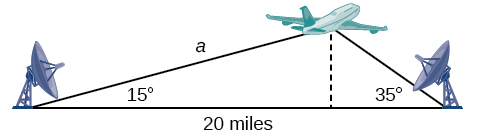
\includegraphics[width=0.6\textwidth]{figs/CNX_Precalc_Figure_08_01_016.jpg}
\end{example}

\newpage
\section*{Exercises}


\begin{exercise}
  Solve for the unknown side and angles. Round your answers to the nearest tenth.\\
  \begin{tikzpicture}
    \tkzDefPoints{0/0/A, 5/0/B}
    \tkzDefTriangle[two angles = 40 and 60](A,B)
    \tkzGetPoint{C}
    \tkzLabelAngle[pos=1.5](B,A,C){$40\degree$}
    \tkzLabelAngle[pos=1.5](C,B,A){$60\degree$}
    \tkzMarkAngle[size=0.8, mark=|](B,A,C)
    \tkzMarkAngle[size=0.8, mark=||](C,B,A)
    \tkzDrawSegments(A,B B,C C,A)
    % \tkzLabelSegment[auto,swap](A,B){$9$}
    \tkzLabelSegment[auto](A,C){$12$}
  \end{tikzpicture}
\end{exercise}

\begin{exercise}
  Solve for the unknown side and angles. Round your answers to the nearest tenth.\\
  \begin{tikzpicture}
    \tkzDefPoints{0/0/A, 6/-1/B}
    \tkzDefTriangle[two angles = 35 and 75](A,B)
    \tkzGetPoint{C}
    \tkzLabelAngle[pos=1](C,B,A){$75\degree$}
    \tkzMarkAngle[size=0.6](C,B,A)
    \tkzDrawSegments(A,B B,C C,A)
    \tkzLabelSegment[auto,swap](A,B){$10$}
    \tkzLabelSegment[auto](A,C){$15$}
  \end{tikzpicture}
\end{exercise}

\newpage

\begin{exercise}
  Find all possible triangles if one side has length $5$ opposite an angle of  $70\degree$, and a second side has length $9$.
\end{exercise}

\begin{exercise}
  Find the area of a triangle shown in the figure below. Round the area to the nearest integer.\\
  \begin{tikzpicture}
    \tkzDefPoints{0/0/A, 5/0/B}
    \tkzDefTriangle[two angles = 40 and 70](A,B)
    \tkzGetPoint{C}
    \tkzLabelAngle[pos=1](B,A,C){$40\degree$}
    \tkzMarkAngle[size=0.6](B,A,C)
    \tkzDrawSegments(A,B B,C C,A)
    \tkzLabelSegment[auto](A,C){$10$}
    \tkzLabelSegment[auto,swap](B,C){$8$}
  \end{tikzpicture}
\end{exercise}

\newpage

\begin{exercise}
  The Figure below shows a satellite orbiting Earth. The satellite passes directly over two tracking stations  $A$ and $B$, which are $69$ miles apart. When the satellite is on one side of the two stations, the angles of elevation at $A$ and $B$ are measured to be $86.2\degree$ and  $83.9\degree$ respectively. How far is the satellite from station  $A$ and how high is the satellite above the ground? Round answers to the nearest whole mile.\\
  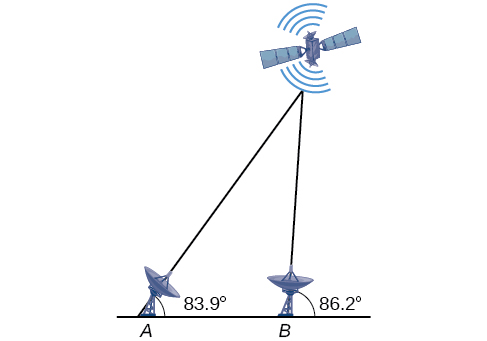
\includegraphics[width=0.6\textwidth]{figs/CNX_Precalc_Figure_08_01_233.jpg}
\end{exercise}

\newpage

\section{Law of Cosine}
\begin{theorem}[Law of Cosine]
  Given a triangle $\triangle ABC$ with sides of lengths $a$, $b$, and $c$ opposite to angles $A$, $B$, and $C$, respectively, then
\[
\begin{aligned}
  a^2=&b^2+c^2-2bc\cos A\\
  b^2=&a^2+c^2-2ac\cos B\\
  c^2=&a^2+b^2-2ab\cos C
\end{aligned}
\qquad\qquad \text{or}\qquad\qquad
\begin{aligned}
  \cos A =&\dfrac{b^2+c^2-a^2}{2bc}\\
  \cos B =&\dfrac{a^2+c^2-b^2}{2ac}\\
  \cos C=&\dfrac{a^2+b^2-c^2}{2ab}.
\end{aligned}
\]
\end{theorem}

\begin{example}
  Find the unknown side and angles of the triangle.\\
  \begin{tikzpicture}
    \tkzDefPoints{0/0/A, 6/0/B}
    \tkzDefTriangle[two angles = 70 and 30](A,B)
    \tkzGetPoint{C}
    \tkzLabelAngle[pos=1](B,A,C){$70\degree$}
    \tkzMarkAngle[size=0.6](B,A,C)
    \tkzDrawSegments(A,B B,C C,A)
    \tkzLabelSegment[auto,swap](A,B){$12$}
    \tkzLabelSegment[auto](A,C){$6$}
  \end{tikzpicture}
\end{example}

\begin{example}
   Find the angles in the triangle. Round your answers to the nearest tenth.\\
    \begin{tikzpicture}
      \tkzDefPoints{0/0/A, 5/-1/B}
      \tkzDefTriangle[two angles = 52 and 68](A,B)
      \tkzGetPoint{C}
      % \tkzLabelAngle[pos=1](C,B,A){$84\degree$}
      % \tkzMarkAngle[size=0.6](C,B,A)
      \tkzDrawSegments(A,B B,C C,A)
      \tkzLabelSegment[auto,swap](A,B){$18$}
      \tkzLabelSegment[auto](A,C){$20$}
      \tkzLabelSegment[auto,swap](B,C){$25$}
    \end{tikzpicture}
\end{example}

\newpage

\begin{example}
  To find the distance across a small lake, a surveyor has taken the measurements shown in the figure below. Find the distance across the lake using this information. Round your answers to the nearest tenth.\\
    \begin{tikzpicture}
      \tkzDefPoints{0/0/A, 5/-2/B}
      \tkzDefTriangle[two angles = 52 and 68](A,B)
      \tkzGetPoint{C}
      \tkzLabelAngle[pos=1](B,A,C){$52\degree$}
      \tkzMarkAngle[size=0.6](B,A,C)
      \tkzDrawSegments(A,B B,C C,A)
      \tkzLabelSegment[auto,swap](A,B){$1800$ ft}
      \tkzLabelSegment[auto](A,C){$2000$ ft}
      \tkzDrawPoints(A,B,C)
      \tkzLabelPoints[left](A)
      \tkzLabelPoints[below](B)
      \tkzLabelPoints[above](C)
      \coordinate (D) at ($(C) + (0,-0.1)$);
      \filldraw[blue!30] plot[smooth, tension=.7, fill=blue] coordinates {(3,0) (4,-0.8) (5,-1.9) (6,-.7) (6.5,-1) (7,0.5) (D) (4,1) (3,0)};
    \end{tikzpicture}
\end{example}

\begin{theorem}[Heron's Formula]
The area of oblique triangles in which sides $a$, $b$, and $c$ are known.
\[\text{Area}=\sqrt{s(s-a)(s-b)(s-c)},\]
where $s=\dfrac{(a+b+c)}{2}$ is one half of the perimeter of the triangle, sometimes called the semi-perimeter.
\end{theorem}

\begin{example}
  Find the area of the triangle in the figure below using Heron's formula.\\
  \begin{tikzpicture}
    \tkzDefPoints{0/0/A, 6/0/B}
    \tkzDefTriangle[two angles = 40 and 30](A,B)
    \tkzGetPoint{C}
    % \tkzLabelAngle[pos=1](B,A,C){$30\degree$}
    % \tkzMarkAngle[size=0.6](B,A,C)
    \tkzDrawSegments(A,B B,C C,A)
    \tkzLabelSegment[auto,swap](A,B){$c=15$}
    \tkzLabelSegment[auto,swap](B,C){$a=10$}
    \tkzLabelSegment[auto](A,C){$b=7$}
  \end{tikzpicture}
\end{example}
\vspace*{-0.1\textheight}

\newpage
\section*{Exercises}


\begin{exercise}
  Find the unknown side and angles of the triangle.\\
  \begin{tikzpicture}
    \tkzDefPoints{0/0/A, 6/0/B}
    \tkzDefTriangle[two angles = 65 and 45](A,B)
    \tkzGetPoint{C}
    \tkzLabelAngle[pos=1](B,A,C){$65\degree$}
    \tkzMarkAngle[size=0.6](B,A,C)
    \tkzDrawSegments(A,B B,C C,A)
    \tkzLabelSegment[auto,swap](A,B){$15$}
    \tkzLabelSegment[auto](A,C){$10$}
  \end{tikzpicture}
\end{exercise}

\begin{exercise}
   Find the angles in the triangle. Round your answers to the nearest tenth.\\
    \begin{tikzpicture}
      \tkzDefPoints{0/0/A, 5/-1/B}
      \tkzDefTriangle[two angles = 50 and 60](A,B)
      \tkzGetPoint{C}
      % \tkzLabelAngle[pos=1](C,B,A){$84\degree$}
      % \tkzMarkAngle[size=0.6](C,B,A)
      \tkzDrawSegments(A,B B,C C,A)
      \tkzLabelSegment[auto,swap](A,B){$22$}
      \tkzLabelSegment[auto](A,C){$18$}
      \tkzLabelSegment[auto,swap](B,C){$25$}
    \end{tikzpicture}
\end{exercise}

\newpage

\begin{exercise}
  To find the distance across a small lake, a surveyor has taken the measurements shown in the figure below. Find the distance across the lake using this information. Round your answers to the nearest tenth.\\
    \begin{tikzpicture}
      \tkzDefPoints{0/0/A, 5/-2/B}
      \tkzDefTriangle[two angles = 62 and 68](A,B)
      \tkzGetPoint{C}
      \tkzLabelAngle[pos=1](B,A,C){$62\degree$}
      \tkzMarkAngle[size=0.6](B,A,C)
      \tkzDrawSegments(A,B B,C C,A)
      \tkzLabelSegment[auto,swap](A,B){$2.1$ km}
      \tkzLabelSegment[auto](A,C){$2.4$ km}
      \tkzDrawPoints(A,B,C)
      \tkzLabelPoints[left](A)
      \tkzLabelPoints[below](B)
      \tkzLabelPoints[above](C)
      \coordinate (D) at ($(C) + (0,-0.1)$);
      \filldraw[blue!30] plot[smooth, tension=.7, fill=blue] coordinates {(3,0) (4,-0.8) (5,-1.9) (6,-.7) (6.5,-1) (7,0.5) (D) (4,1) (3,0)};
    \end{tikzpicture}
\end{exercise}

\begin{exercise}
  Find the area of the triangle in the figure below using Heron's formula.\\
  \begin{tikzpicture}
    \tkzDefPoints{0/0/A, 6/0/B}
    \tkzDefTriangle[two angles = 55 and 62](A,B)
    \tkzGetPoint{C}
    % \tkzLabelAngle[pos=1](B,A,C){$30\degree$}
    % \tkzMarkAngle[size=0.6](B,A,C)
    \tkzDrawSegments(A,B B,C C,A)
    \tkzLabelSegment[auto,swap](A,B){$c=20$}
    \tkzLabelSegment[auto,swap](B,C){$a=15$}
    \tkzLabelSegment[auto](A,C){$b=12$}
  \end{tikzpicture}
\end{exercise}
